\documentclass[11pt]{article}
\usepackage{graphicx}

\begin{document}

{\bf  Scientific Justification:} {\sl Type Ia supernovae (SNe~Ia) are thermonuclear explosions of white dwarfs in a binary system. Their use as distance indicators in cosmology has led to dedicated efforts to obtain data for large samples of SNeIa. This has revealed a heterogeneity in the photometric and spectroscopic properties of the explosions. However, most of the assimilated data for the SNe~Ia are directed towards understanding them during the early photospheric phase. At late phases, the $\gamma$ ray escape fraction increases and most of the light curve is powered by the positrons. Hence, these late-phases of these SNe offer other opportunities to study the physics of these explosions.

At phases greater than $\sim$ 150 days past maximum light, the light curves are powered by the deposition of positron kinetic energy. The fraction of positron energy deposited into the ejecta is thought to depend on the magnetic field configuration, with a stronger magnetic field leading to higher fraction of positrons being trapped. Thus, the late-time (pseudo-)bolometric light curve (integrated from filters u to K) is an efficient tool in constraining the nature of the magnetic field in the SNe and, in principle can constrain the contribution these positrons make to the galactic 511 keV line.  In figure \ref{fig:bol}, we can see the (pseudo-)bolometric light curve for SN2001el from Stritzinger $\&$ Sollerman 2007, compared to their toy model. Their bolometric light curve only extends out to $\sim$  +440 days.

A few recent studies have shown that SNeIa show a flattening of the Near Infrared (NIR) light curve at a few hundred days past maximum light . This is attributed to a flux redistribution at late epochs from the optical to the NIR. However, there objects with such late time data have very sparse sampling and no coverage beyond $\sim$ +700 days. 

SN2014J, the nearest supernova in the past 4 decades provides a unique laboratory to study this late time behaviour. Dedicated near-maximum observations have led to epochal discoveries, like the first observation of the $^{56}Co$ line in the $\gamma$ rays.  Its proximity means that it is bright, even at late epochs $\geq$ +700 days, which allows us to probe the physics of the explosion out to later epochs than current studies. A time sampling of observations every $\sim$ 30-50 days within the range of +300-+800 days would allow us to constrain the nature of this late time decline in the NIR precisely. Observations post +700 days will allow us to observe the behaviour of SNeIa in the NIR at very late epochs, to constrain when the flattening ends and what the nature of the light curve is at $>$ +700 days. 

Very late time NIR observations also allow constraints on the occurrence of an Infrared Catastrophe (IRC) in the ejecta. From a modelling point of view, the IRC is expected to occur once the ejecta temperature drops below a threshold. For SN2003hv, it has been seen that there in no drop in luminosity in the NIR which suggests that at least part of the ejecta is above the temperature threshold. Observations with regular time sampling in the phase range between +550 and $\geq$ +700 days will allow strong constraints on the occurrence of an IRC in 2014J. An absence of the IRC in the given phase range can be explained by the clumping of the ejecta in particular regions, which would postpone the onset of the IRC. Hence, observations at $\geq$ +700 are crucial to understanding to understanding the signatures of an IRC. 

\begin{figure}
	\centering
	
	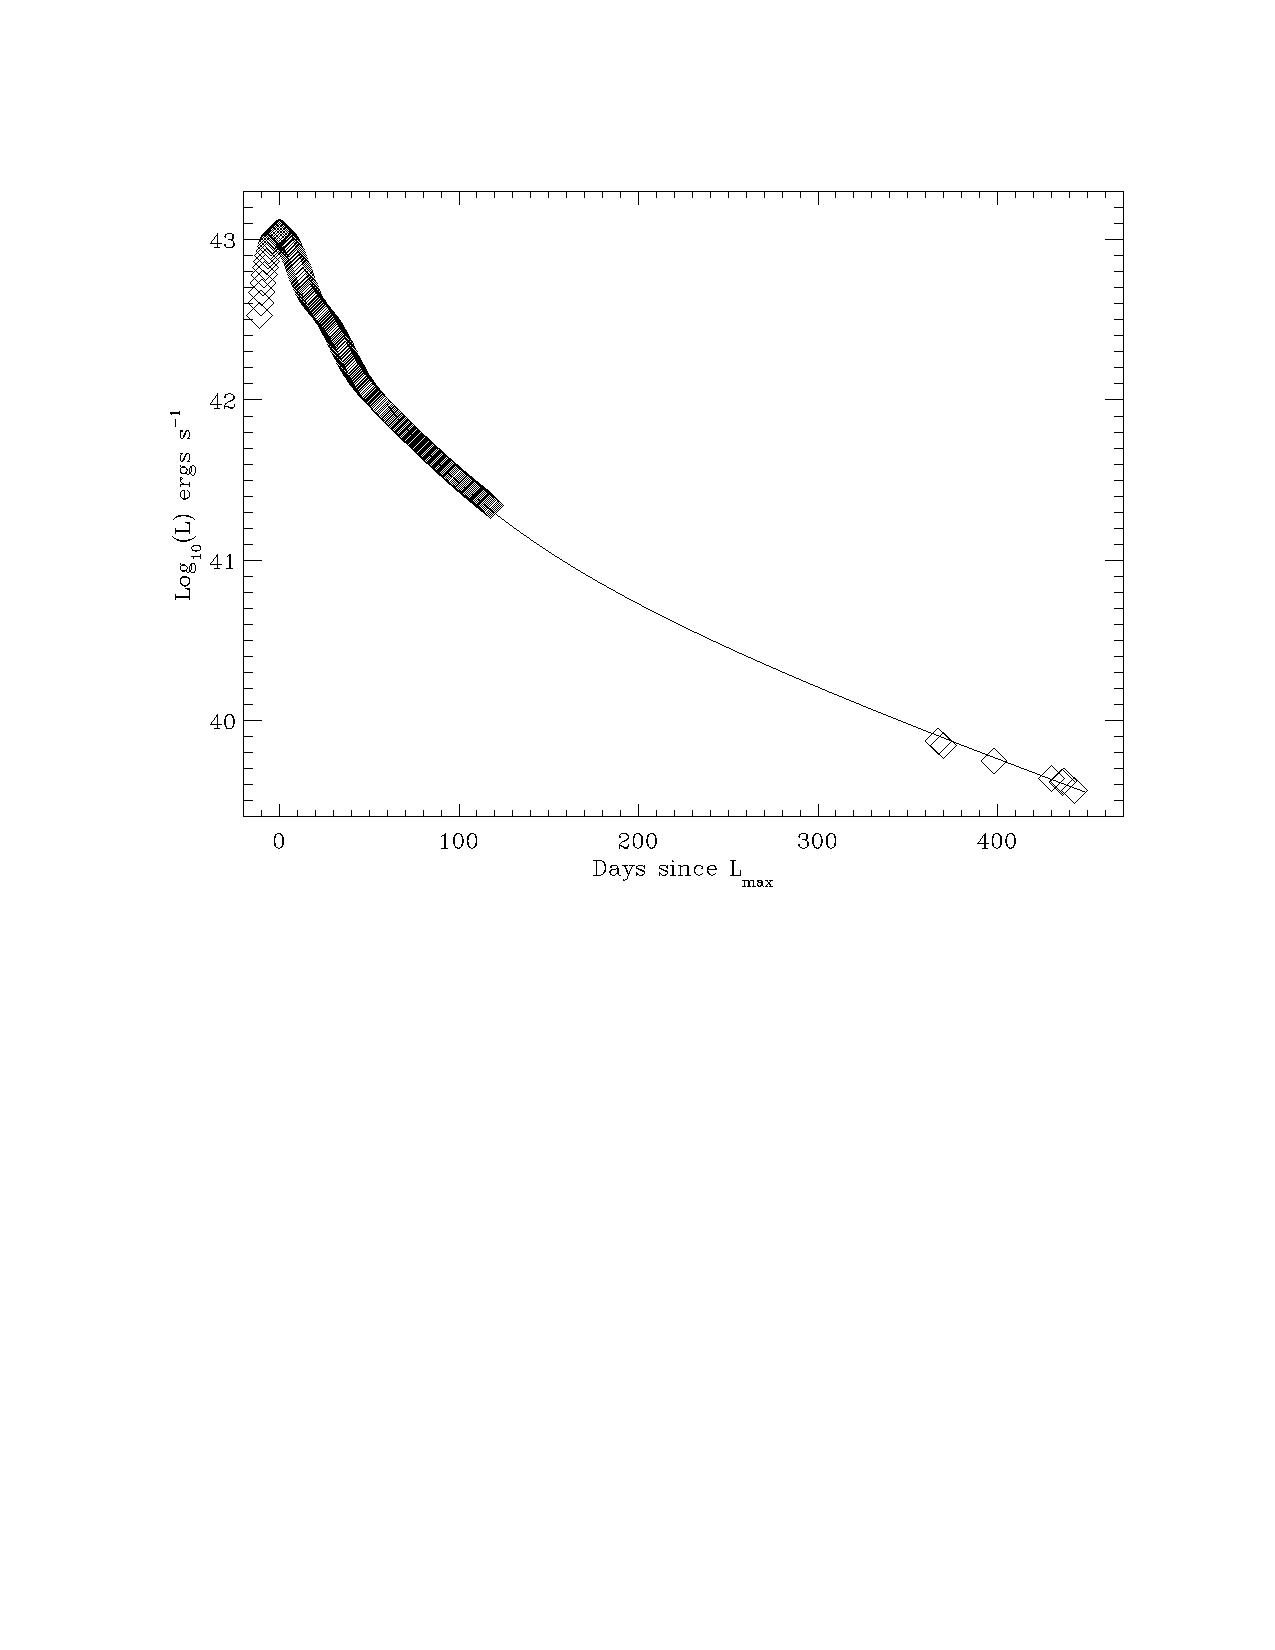
\includegraphics[width=.5\textwidth]{hct_files/sn01el_bol.pdf}
	\caption{(Pseudo-) bolometric light curve of SN2001el from Stritzinger $\&$ Sollerman 2007}
	\label{fig:bol}
\end{figure}
\end{document}